% Same legend as in the paper (Overleaf). Source: DFUDA paper \tsnelegend.
% Used as the layout reference for tools/render_tsne_readme_figure.py
%
% tsne_colorbar
\newcommand{\tsnelegend}{
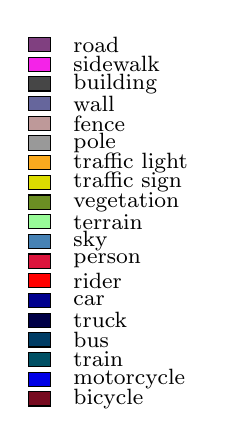
\begin{tikzpicture}[font=\fontsize{8}{7}\selectfont]
\def\xbox{0}
\def\xtext{0.45}
\def\dy{0.25}

\foreach \name/\r/\g/\b/\i in {
road/128/64/128/0,
sidewalk/244/35/232/1,
building/70/70/70/2,
wall/102/102/156/3,
fence/190/153/153/4,
pole/153/153/153/5,
traffic light/250/170/30/6,
traffic sign/220/220/0/7,
vegetation/107/142/35/8,
terrain/152/251/152/9,
sky/70/130/180/10,
person/220/20/60/11,
rider/255/0/0/12,
car/0/0/142/13,
truck/0/0/70/14,
bus/0/60/100/15,
train/0/80/100/16,
motorcycle/0/0/230/17,
bicycle/119/11/32/18
}{
  \definecolor{legendcolor\i}{RGB}{\r,\g,\b}
  \filldraw[draw=black, fill=legendcolor\i] 
    (\xbox,-\i*\dy) rectangle ++(0.28,0.18);
  \node[anchor=west] at (\xtext,-\i*\dy+0.09) {\name};
}
\end{tikzpicture}
}
